\chapter{Zahlenbereiche}
\section{Natürliche Zahlen}
Die natürlichen Zahlen 1, 2, 3, 4, \ldots ~sind die ältesten Zahlen, die sich aus dem Zählen von Gegenständen entwickelt haben.
Dabei nimmt man an, dass man immer weiterzählen kann.\\

\begin{defn}{Natürliche Zahlen}
	Die Menge der natürlichen Zahlen wird mit $\N$ bezeichnet.
	Man schreibt:
	\begin{align*} 
	 \N = \{ 1, 2, 3, 4, \ldots \}\, .
	\end{align*}
	Die Zahlen $1, 2, 3, 4, \ldots$ heissen \emph{Elemente} der Menge $\N$.
	Ist eine Zahl $n$ eine natürliche Zahl, so schreibt man: $n\in\N$\,.
\end{defn}

\vspace{.5cm}
\begin{wrapfigure}{r}{6cm}
	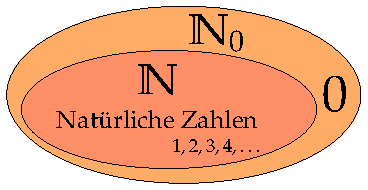
\includegraphics[width=\linewidth]{numberset-naturals-N0}
\end{wrapfigure}
Das Zeichen \glqq $\in$\grqq~bedeutet: \glqq ist Element von\grqq, das Zeichen \glqq $\notin$\grqq~bedeutet: \glqq ist \emph{nicht} Element von\grqq.

\paragraph{Achtung!}
Die Zahl 0 wird dabei {\bfseries nicht} mit dazu genommen.
Wir schreiben:
\begin{align*}
  0 \notin \N\, .
\end{align*}
Möchte man die Null mit einschliessen, so verwenden wir die Schreibweise $\N_0$.\\

\begin{defn}{Natürliche Zahlen zusammen mit Null}
	Die Menge der natürlichen Zahlen wird mit $\N_0$ bezeichnet.
	Man schreibt: $\N_0 = \{ 0, 1, 2, 3, 4, \ldots \}$\,.
\end{defn}

\begin{example}
  Schreibe in das Symbol \relationBox das richtige Zeichen $\in$ oder $\notin$ hinein.
  \begin{align*}
   2 \relationBox \N_0\,,\qquad
   \frac{1}{2} \relationBox \N\,,\qquad
   0 \relationBox \N\,,\qquad
   0 \relationBox \N_0\,,\qquad
   \frac{72}{36} \relationBox \N\,.
  \end{align*}

\end{example}


\vspace{.5cm}
Die natürlichen Zahlen braucht man z.B. um Anzahlen anzugeben, Rangplätze oder Reihenfolgen festzulegen oder (bestimmte) Messergebnisse festzuhalten.

\begin{example}~
	\begin{itemize}\setlength\itemsep{0pt}
		\item Wir haben heute 6 Lektionen. (Anzahl)
		\item Heute ist der erste Tag des Monats. (Rangplatz)
		\item Heute ist es 30 Grad warm. (Messergebnis)
	\end{itemize}
\end{example}

Man kann mit den natürlichen Zahlen auch (bestimmte) Gleichungen lösen.
\begin{example}
 Heute ist es \unit[30]{°C} warm und damit \unit[2]{°C} wärmer als gestern.
 D.h. für die Temperatur $x$ von gestern in \unit{°C} gilt die Gleichung:
 \begin{align*}
   x + 2 = 30
 \end{align*}
Die Lösung der Gleichung ist eine natürliche Zahl, nämlich $x = 28$\,, d.h. die gesuchte Temperatur ist \unit[28]{°C}
\end{example}


\section{Negative ganze Zahlen}
\begin{wrapfigure}{r}[1cm]{5cm}
 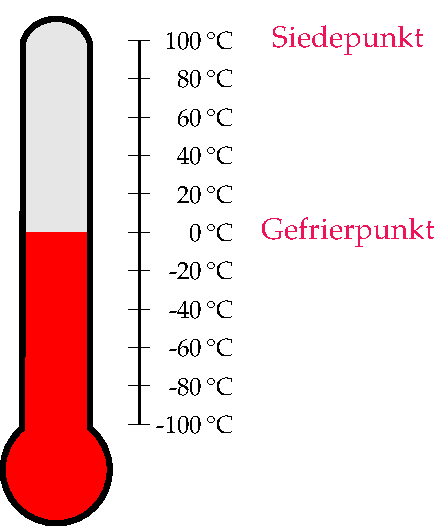
\includegraphics[width=\linewidth]{thermometer}
\end{wrapfigure}
Für viele Zwecke reichen die natürlichen Zahlen nicht aus.
Ist es heute z.B. \unit[30]{°C} warm und wir wollen es mit der Temperatur vor einem halben Jahr vergleichen, so stellen wir vielleicht fest, dass es heute \unit[35]{°C} wärmer ist als vor einem halben Jahr.
D.h. die Temperatur $x$ vor einem halben Jahr in \unit{°C} erfüllt die Gleichung:
\begin{align*}
	x + 35 = 30
\end{align*}
Diese Gleichung lässt sich nicht mit den natürlichen Zahlen lösen, wohl aber, wenn wir negative Zahlen zulassen.
Dann erhalten wir: $x = -5$\,, d.h. die Temperatur ist \unit[--5]{°C}\,.

\subsection{Weitere Beispiele}
Die folgenden Beispiele zeigen, dass im Alltag negative Zahlen oft in Verbindung mit einer künstlich festgelegten Null vorkommen.

\paragraph{Temperatur.}
In Europa misst man die Temperatur in \unit{°C}.
Diese Temperaturskala ist so definiert, dass bei Normaldruck der Gefrierpunkt des Wasser gleich \unit[0]{°C} entspricht und der Siedepunkt gleich \unit[100]{°C}.
Wenn eine Temperatur also unter der Temperatur des Wassergefrierpunkts ist, so ist sie negativ.

\paragraph{Meter über dem Meeresspiegel.}
Auf Landkarten wird die Höhe z.B. in Metern über dem Meeresspiegel (m ü.M.) angegeben.
Zum Beispiel liegt der Gipfel des Mt. Whitney in den USA \unit[4418]{m} über dem Meer, kurz \unit[4418]{m ü.M.}
Dabei wurde der Meeresspiegel künstlich als \emph{Normalhöhe} festgelegt.
Dies führt dazu, dass das sogenannte \emph{Tal des Todes} sich bei \unit[-86]{m ü.M.} befindet.

\subsection{Zahlengerade}
\begin{figure}[H]
	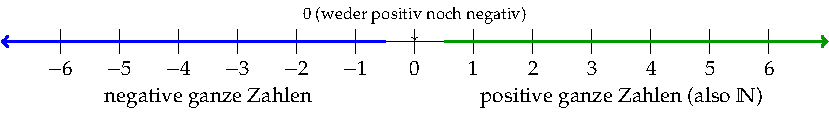
\includegraphics[width=\linewidth]{zahlengerade}
	\caption{Die Zahlengerade mit den positiven ganzen Zahlen rechts von der Null und den negativen ganzen Zahlen links von der Null.
	Die Null ist weder positiv noch negativ.}
	\label{fig:zahlengerade-pos-neg}
\end{figure}

Die sogenannten negativen ganzen Zahlen $-1, -2, -3, \ldots$ stehen links von 0 auf der Zahlengeraden, siehe Abbildung \ref{fig:zahlengerade-pos-neg}.
Die natürlichen Zahlen, die auch positive ganze Zahlen genannt werden, stehen rechts von Null auf der Zahlengeraden. Beachte, dass die Null selbst weder positiv noch negativ ist.
Möchtest du die Zahlen in $\N_0$ auf diese Weise bezeichnen (also die Null mit einschliessen), so kannst du sie nicht-negative ganze Zahlen nennen.

\section{Ganze Zahlen}
\begin{wrapfigure}{r}{7cm}
	\vspace{-1cm}
	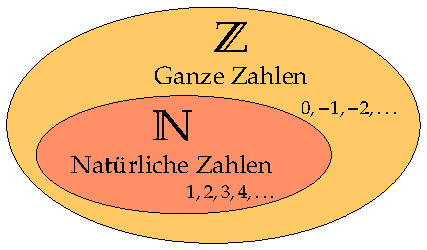
\includegraphics[width=\linewidth]{numberset-integers}
	% \caption{Die natürlichen Zahlen sind in den ganzen Zahlen enthalten.
	% Auf eine Darstellung der Menge $\N_0$ wurde hier für die bessere Übersicht verzichtet.}
	% \label{fig:numberset-integers}
	\vspace{-2cm}
\end{wrapfigure}
Die Menge der ganzen Zahlen besteht aus den natürlichen Zahlen, den negativen ganzen Zahlen und der Null.

Jede natürliche Zahl ist auch eine ganze Zahl, aber nicht andersherum.
D.h. die Menge der natürlichen Zahlen ist komplett in der Menge der ganzen Zahlen enthalten.
%, siehe Abbildung \ref{fig:numberset-integers}.

\vspace{1cm}
\begin{defn}{Ganzen Zahlen}
	Fügt man zu den natürlichen Zahlen $\N$ die Zahl 0 und die negativen ganzen Zahlen $-1, -2, -3,\ldots$ hinzu,
	so erhält man die Menge der ganzen Zahlen $\Z = \{ \ldots, -3, -2, -1, 0, 1, 2, 3, \ldots \}$\, .
\end{defn}


\subsection{Regeln}
Für das Rechnen mit den ganzen Zahlen gelten die arithmetischen Grundgesetze von Seite \pageref{law:arithmetic}, bis auf eine Ausnahme!
Welche? (Schreibe es selber auf.)\\
\kariert{15}{2}\\~\\
Vervollständige die Übersicht von Seite \pageref{law:arithmetic} für alle Regeln bis auf die, die nicht gilt:
\begin{law}{Arithmetische Grundgesetze für \underline{\bfseries die ganzen Zahlen}}
    \bgroup
    \def\arraystretch{2.5}
	\begin{tabularx}{\linewidth}{|X|p{3.7cm}|p{3.7cm}|}
			\hline
			 & Addition & Multiplikation \\
			\hline
			Kommutativgesetz &  &  \\\hline
			Assoziativgesetz &  &  \\\hline
			Es gibt Neutralelement\newline 0 bzw. 1\,. &  &  \\\hline
			Es gibt inverses Element\newline~ & & \\
			\hline
			Distributivgesetz & \multicolumn{2}{c|}{} \\
			\hline
    \end{tabularx}
    \egroup
\end{law}

\subsection{Subtraktion}
Mithilfe der negativen Zahlen kann man die Subtraktion als eine Addition mit einer negativen Zahl schreiben und so die Rechenregeln, die für die Addition gelten, anwenden, wie z.B. das Kommutativgesetz und das Assoziativgesetz.
\begin{example} Kommutativgesetz der Addition:
	\begin{align*}
					8 - 5		&\,=\, 8 + (-5) \,=\, (-5) + 8\\
		\text{Aber:}\quad 8 - 5		&\,\neq\, 5 - 8
	\end{align*}
	Wende das Kommutativgesetz einmal nach dem gleichen Schema selbst an:\\
	\kariert[\large 10 -- 3 \,=\,]{15}{1.5}\\
\end{example}
\begin{example} Assoziativgesetz der Addition:
	\begin{align*}
					(8 - 5) - 1			&\,=\, \bigl(8 + (-5)\bigr) + (-1) \,=\, 8 + \bigl( (-5) + (-1)\bigr)\\
		\text{Aber:}\quad (8 - 5) - 1	&\,\neq\, 8 - (5 - 1)
	\end{align*}
	Wende das Assoziativgesetz einmal nach dem gleichen Schema selbst an:\\
	\kariert[\large (10 -- 3) -- 2 \,=\,]{15}{2}\\
\end{example}
\begin{example} Minusklammer:
	\begin{align*}
					1 -(8 - 5)			&\,=\, 1 + (-1)\cdot\bigl(8 + (-5)\bigr)\,=\, 1 + (-1)\cdot 8 + (-1)\cdot (-5) = 1 - 8 + 5\\
	\end{align*}
	Wende die Minusklammer einmal nach dem gleichen Schema selbst an:\\
	\kariert[\large 10 -- (3 -- 2) \,=\,]{15}{2}\\
\end{example}

\section{Rationale Zahlen}
\begin{defn}{Rationale Zahlen}
	Die Menge der rationalen Zahlen $\Q$ besteht aus allen Zahlen, die man als Bruch schreiben kann.
	\begin{align*}
		\Q = \left\{\left. \frac{p}{q} ~\right|~ p,q \in \Z;~ q \neq 0\, \right\}
	\end{align*}
	
\end{defn}


% \section{Kann man alle Zahlen als Bruch darstellen?}
% Hier muss noch etwas Geschichte hin.

